%% Font size %%
\documentclass[11pt]{article}

%% Load the custom package
\usepackage{Mathdoc}

%% Numéro de séquence %% Titre de la séquence %%
\renewcommand{\centerhead}{S04 - Les angles}


\usetikzlibrary{calc}
% Angle de sommet V : \angleCours[échelle]{mesure}{rotation}{L1}{V}{L2}
\newcommand{\angleCours}[6][1]{%
  \begin{tikzpicture}[scale=#1,baseline=(V.base)]
    \coordinate (V) at (0,0);
    \ifnum#2=90
      \draw[gray!70!black, fill=gray!25] (0,0) -- (#3:3mm)
        -- ($(#3:3mm)+({#3+90}:3mm)$) -- ({#3+90}:3mm) -- cycle;
    \else\ifnum#2>0
      \draw[gray!70!black, fill=gray!25] (0,0) -- (#3:4.5mm)
        arc[start angle=#3, delta angle=#2, radius=4.5mm] -- cycle;
    \fi\fi
    \draw[thick] (#3:1.6) -- (V) -- ({#3+#2}:1.6);
    \foreach \a in {#3,{#3+#2}} \draw (\a:1.2) ++(-1.5pt,-1.5pt) -- ++(3pt,3pt) ++(-3pt,0) -- ++(3pt,-3pt);
    \node at (#3:1.2) [shift={({#3-90}:2.5mm)}] {$#4$};
    \node at ({#3+#2/2+180}:3.5mm) {$#5$};
    \node at ({#3+#2}:1.2) [shift={({#3+#2+90}:2.5mm)}] {$#6$};
  \end{tikzpicture}%
}
% Encadré « compétence » en tête de partie
\newcommand{\comp}[2]{\par\smallskip\noindent\colorbox{gray!15}{\parbox{\dimexpr\linewidth-2\fboxsep}{\small\textbf{Compétence #1} : #2}}\par\smallskip}

%% Spacing commands %%
\renewcommand{\baselinestretch}{1} \setlength{\parindent}{0pt}

\begin{document}

\begin{tcolorbox}[colback=white,colframe=black,boxrule=0.6pt,arc=2mm,title={\textbf{Ce que je dois savoir faire à la fin du chapitre}},coltitle=black,colbacktitle=gray!15]
\begin{tabular}{@{}ll@{}}
\textbf{6C04-GEO10} & \textbf{Nommer} un angle \hfill (partie 1)\\
\textbf{6C04-GEO11} & Donner le \textbf{sommet} et les \textbf{côtés} d'un angle \hfill (partie 1)\\
\textbf{6C04-GEO12} & Reconnaître la \textbf{nature} d'un angle (nul, aigu, droit, obtus, plat) \hfill (partie 2)\\
\textbf{6C04-GEO13} & \textbf{Classer} des angles selon leur nature \hfill (partie 2)\\
\textbf{6C04-GEO14} & \textbf{Mesurer} un angle au rapporteur \hfill (partie 3)\\
\textbf{6C04-GEO15/16} & \textbf{Construire} un angle de mesure donnée \hfill (partie 4)\\
\end{tabular}
\end{tcolorbox}

\section{Vocabulaire : nommer un angle}

\begin{definition}
Deux \textbf{demi-droites de même origine} forment un \textbf{angle}.
\end{definition}

\subsection{Sommet et côtés}
\comp{6C04-GEO11}{donner le sommet et les côtés d'un angle \hfill \textit{Fiche Ex-6C04-04}}

\begin{vocabulaire}
\begin{itemize}
\item L'origine commune des deux demi-droites est le \textbf{sommet} de l'angle (c'est un \textbf{point}).
\item Les deux demi-droites sont les \textbf{côtés} de l'angle. Elles commencent au sommet :
on écrit le sommet \textbf{en premier}, avec un crochet : $[BA)$, $[BC)$.
\end{itemize}
\end{vocabulaire}

\begin{center}
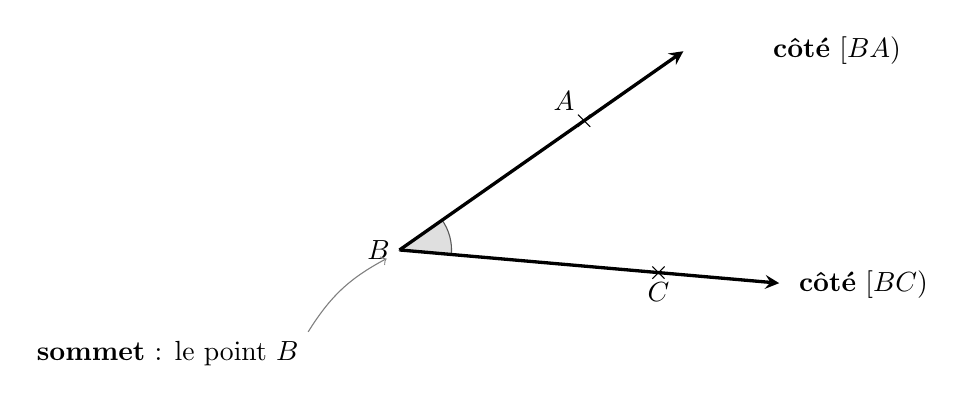
\begin{tikzpicture}[scale=1.1]
  \coordinate (B) at (0,0); \coordinate (A) at (35:2.6); \coordinate (C) at (-5:3);
  \draw[gray!70!black, fill=gray!25] (B) -- (-5:6mm) arc[start angle=-5, delta angle=40, radius=6mm] -- cycle;
  \draw[very thick,->,>=stealth] (B) -- (35:4);
  \draw[very thick,->,>=stealth] (B) -- (-5:4.4);
  \foreach \P in {A,C} \draw (\P) ++(-2pt,-2pt) -- ++(4pt,4pt) ++(-4pt,0) -- ++(4pt,-4pt);
  \node[above left] at (A) {$A$}; \node[below] at (C) {$C$}; \node[left] at (B) {$B$};
  \node[anchor=west,align=left] (s) at (-4.3,-1.2) {\textbf{sommet} : le point $B$};
  \draw[->,gray] (s.north east) to[bend left=15] (-0.15,-0.1);
  \node[anchor=west,align=left] at (4.2,2.3) {\textbf{côté} $[BA)$};
  \node[anchor=west,align=left] at (4.5,-0.4) {\textbf{côté} $[BC)$};
\end{tikzpicture}
\end{center}

\subsection{Nommer un angle}
\comp{6C04-GEO10}{nommer un angle avec trois lettres \hfill \textit{Fiche Ex-6C04-03}}

\begin{notation}
Pour nommer un angle, on écrit \textbf{trois lettres} sous un \textbf{chapeau} : $\widehat{ABC}$.
\begin{itemize}
\item la lettre \textbf{du milieu} est \textbf{le sommet} ;
\item les deux autres lettres sont des points, \textbf{un sur chaque côté}.
\end{itemize}
\end{notation}

\begin{exemple}
L'angle de la figure ci-dessus se note $\widehat{ABC}$ ou $\widehat{CBA}$ (même angle : le sommet $B$ reste au milieu).\\
Son sommet est le point $B$, ses côtés sont les demi-droites $[BA)$ et $[BC)$.
\end{exemple}

\begin{remarque}
\textbf{Attention :} $\widehat{BAC}$ n'est \textbf{pas} le même angle : son sommet est $A$ ! \\
Si plusieurs points sont sur un même côté, l'angle a plusieurs noms : si $D \in [BA)$, alors $\widehat{ABC} = \widehat{DBC}$.
\end{remarque}

\section{Nature d'un angle : les angles particuliers}
\comp{6C04-GEO12 et GEO13}{reconnaître la nature d'un angle, classer des angles \hfill \textit{Fiches Ex-6C04-05 et 06}}

\begin{definition}
Il y a \textbf{cinq} angles particuliers à connaître : l'angle \textbf{nul}, l'angle \textbf{aigu}, l'angle \textbf{droit},
l'angle \textbf{obtus} et l'angle \textbf{plat}. Pour trouver la nature d'un angle, on le compare à l'\textbf{angle droit}
(codé par un petit carré) et à l'\textbf{angle plat}.
\end{definition}

\begin{center}
\renewcommand{\arraystretch}{1.3}
\begin{tabularx}{\linewidth}{|>{\centering\arraybackslash}m{1.9cm}|*{5}{>{\centering\arraybackslash}X|}}
\hline
\textit{Nom} & \textbf{Angle nul} & \textbf{Angle aigu} & \textbf{Angle droit} & \textbf{Angle obtus} & \textbf{Angle plat} \\ \hline
\textit{Figure} &
\angleCours[0.8]{0}{10}{A}{O}{B} &
\angleCours[0.8]{40}{10}{A}{O}{B} &
\angleCours[0.8]{90}{10}{A}{O}{B} &
\angleCours[0.8]{135}{10}{A}{O}{B} &
\angleCours[0.8]{180}{0}{A}{O}{B} \\ \hline
\textit{Je le reconnais} &
Les deux côtés sont confondus &
Plus \textbf{petit} qu'un angle droit &
Il est codé par un \textbf{petit carré} &
Plus \textbf{grand} qu'un angle droit, plus petit qu'un plat &
Les côtés sont dans le prolongement : $A$, $O$, $B$ \textbf{alignés} \\ \hline
\textit{Mesure} & $0\degre$ & entre $0\degre$ et $90\degre$ & $90\degre$ & entre $90\degre$ et $180\degre$ & $180\degre$ \\ \hline
\end{tabularx}
\end{center}

\begin{remarque}
Un angle droit, c'est la \textbf{moitié} d'un angle plat : $180\degre \div 2 = 90\degre$.
\end{remarque}

\begin{exercice}[0][Exercice traité : reconnaître et classer]
\textbf{Méthode :} je compare l'angle à un angle droit.
\begin{itemize}
\item Les deux côtés sont \textbf{confondus} $\to$ l'angle est \textbf{nul}.
\item Il est \textbf{plus petit} qu'un angle droit $\to$ \textbf{aigu} ;\quad codé par un \textbf{petit carré} $\to$ \textbf{droit}.
\item Il est \textbf{plus grand} qu'un angle droit $\to$ \textbf{obtus} ;\quad les points sont \textbf{alignés} $\to$ \textbf{plat}.
\end{itemize}
\textbf{Classer les mesures} $35\degre$ ; $90\degre$ ; $150\degre$ ; $180\degre$ ; $89\degre$ ; $91\degre$ ; $0\degre$ :
\begin{center}
\renewcommand{\arraystretch}{1.3}
\begin{tabular}{|c|c|c|c|c|}
\hline
\textbf{Nul} & \textbf{Aigus} & \textbf{Droit} & \textbf{Obtus} & \textbf{Plat} \\ \hline
$0\degre$ & $35\degre$ ; $89\degre$ & $90\degre$ & $150\degre$ ; $91\degre$ & $180\degre$ \\ \hline
\end{tabular}
\end{center}
\textit{Piège :} $89\degre$ et $91\degre$ sont tout près de l'angle droit, mais le premier est aigu et le second obtus.
\end{exercice}

\newpage
\section{Mesurer un angle}
\comp{6C04-GEO14}{mesurer un angle au rapporteur}

\begin{definition}
L'unité de mesure des angles est le degré, noté "$\degre$" \\ Pour mesurer un
angle on peut utiliser un rapporteur
\end{definition}

\begin{multicols}{2}
\encart{5cm}
\columnbreak
\begin{itemize}[label=\textbullet]
\item On lit la mesure de l'angle $\widehat{FCE}$ sur les \textbf{graduations extérieures}. \\ $\widehat{FCE}=50$° 
\item On lit la mesure de l'angle $\widehat{DCE}$ sur les \textbf{graduations intérieures}. \\ $\widehat{DCE}=130$° 
\end{itemize}
\end{multicols}


\begin{multicols}{2}
Deux angles de même mesure sont codés de la même façon. $\widehat{IHJ}=\widehat{KML}$
\begin{tikzpicture}[line cap=round,line join=round,>=triangle 45,x=2cm,y=2cm]
\clip(-0.5,-1) rectangle (3.5,1);
\draw [shift={(0,0)},line width=1pt,fill=black,fill opacity=0.10000000149011612] (0,0) -- (0:0.47730452283397756) arc (0:26.56505117707799:0.47730452283397756) -- cycle;
\draw [shift={(3,-0.5)},line width=1pt,fill=black,fill opacity=0.10000000149011612] (0,0) -- (180:0.47730452283397756) arc (180:206.565051177078:0.47730452283397756) -- cycle;
\draw [shift={(0,0)},line width=1pt] (0:0.47730452283397756) arc (0:26.56505117707799:0.47730452283397756);
\draw[line width=1pt] (0.4343674562627567,0.1240527944935223) -- (0.48354113055665376,0.13809650707769497);
\draw[line width=1pt] (0.4439881600241419,0.08329883936890714) -- (0.49425097059291273,0.09272889665595326);
\draw [line width=1pt] (1.5,0)-- (0,0);
\draw [line width=1pt] (0,0)-- (1,0.5);
\draw [line width=1pt] (1.5,-0.5)-- (3,-0.5);
\draw [line width=1pt] (3,-0.5)-- (2,-1);
\draw [shift={(3,-0.5)},line width=1pt] (180:0.47730452283397756) arc (180:206.565051177078:0.47730452283397756);
\draw[line width=1pt] (2.565632543737243,-0.6240527944935229) -- (2.5164588694433463,-0.6380965070776952);
\draw[line width=1pt] (2.5560118399758576,-0.5832988393689074) -- (2.5057490294070868,-0.5927288966559535);
\begin{scriptsize}
\draw [color=black] (0,0)-- ++(-2.5pt,-2.5pt) -- ++(5pt,5pt) ++(-5pt,0) -- ++(5pt,-5pt);
\draw[color=black] (-0.1433995465088165,-0.021089601039946962) node {$H$};
\draw [color=black] (3,-0.5)-- ++(-2.5pt,-2.5pt) -- ++(5pt,5pt) ++(-5pt,0) -- ++(5pt,-5pt);
\draw[color=black] (3.0545407564788327,-0.3552027670237303) node {$M$};
\draw [color=black] (0.7100818465242826,0.3550409232621413)-- ++(-2.5pt,-2.5pt) -- ++(5pt,5pt) ++(-5pt,0) -- ++(5pt,-5pt);
\draw[color=black] (0.7634790468757408,0.5039453740774268) node {$I$};
\draw [color=black] (1.0225872164141856,0)-- ++(-2.5pt,-2.5pt) -- ++(5pt,5pt) ++(-5pt,0) -- ++(5pt,-5pt);
\draw[color=black] (1.0771363047380689,0.14937629997218738) node {$J$};
\draw [color=black] (2.065838530608451,-0.5)-- ++(-2.5pt,-2.5pt) -- ++(5pt,5pt) ++(-5pt,0) -- ++(5pt,-5pt);
\draw[color=black] (2.120387618932334,-0.3552027670237303) node {$K$};
\draw [color=black] (2.3801398052902196,-0.8099300973548902)-- ++(-2.5pt,-2.5pt) -- ++(5pt,5pt) ++(-5pt,0) -- ++(5pt,-5pt);
\draw[color=black] (2.434044876794662,-0.6620413888455722) node {$L$};
\end{scriptsize}
\end{tikzpicture}
\end{multicols}

\begin{remarque}
Rappel (partie 2) : \textbf{l'angle droit} mesure $90\degre$
et \textbf{l'angle plat} mesure $180\degre$.
\end{remarque}

\newpage
\section{Construire un angle}
\comp{6C04-GEO15/16}{construire un angle de mesure donnée}

\textbf{Énoncé :} Tracer un angle $\widehat{BAC}$ de mesure $137$°.

\begin{multicols}{2}
\makebox[\linewidth]{} \\ \makebox[\linewidth]{} \\ 
\noindent \textbf{Étape 1 :} Le sommet de l'angle est A, il faut donc commencer par tracer la demie-droite [AB) (par exemple), et placer le rapporteur afin d'avoir le "0" de la graduation sur la demie-droite [AB). \\
\begin{tikzpicture}[line cap=round,line join=round,>=triangle 45,x=1cm,y=1cm]
\clip(-3.5,-3.5) rectangle (3.5,3.5);
\draw [line width=1pt] (-3,-3)-- (-3,3);
\draw [line width=1pt] (-3,3)-- (3,3);
\draw [line width=1pt] (3,3)-- (3,-3);
\draw [line width=1pt] (3,-3)-- (-3,-3);
\draw [line width=1pt] (-2.5,-1)-- (0,-1);
\begin{scriptsize}
\draw [color=black] (0,-1)-- ++(-2.5pt,-2.5pt) -- ++(5pt,5pt) ++(-5pt,0) -- ++(5pt,-5pt);
\draw[color=black] (0.4352289909462427,-1.351713241466346) node {$A$};
\draw [color=black] (-2,-1)-- ++(-2.5pt,-2.5pt) -- ++(5pt,5pt) ++(-5pt,0) -- ++(5pt,-5pt);
\draw[color=black] (-1.9016326821732072,-1.6343981212791856) node {$B$};
\end{scriptsize}
\end{tikzpicture}
\end{multicols}

\begin{multicols}{2}
\makebox[\linewidth]{} \\ \makebox[\linewidth]{} \\ \makebox[\linewidth]{} \\ 
\noindent \textbf{Étape 2 :} Comme la graduation "0" est sur l’extérieur, on cherche la mesure $137$° sur la \textbf{ligne extérieure}, puis on fait une marque au crayon.  \\
\begin{tikzpicture}[line cap=round,line join=round,>=triangle 45,x=1cm,y=1cm]
\clip(-3.5,-3.5) rectangle (3.5,3.5);
\draw [line width=1pt] (-3,-3)-- (-3,3);
\draw [line width=1pt] (-3,3)-- (3,3);
\draw [line width=1pt] (3,3)-- (3,-3);
\draw [line width=1pt] (3,-3)-- (-3,-3);
\draw [line width=1pt] (-2.5,-1)-- (0,-1);
\draw [line width=1pt] (0,-1)-- (1.889297573418096,0.7617984894156513);
\begin{scriptsize}
\draw [color=black] (0,-1)-- ++(-2.5pt,-2.5pt) -- ++(5pt,5pt) ++(-5pt,0) -- ++(5pt,-5pt);
\draw[color=black] (0.4352289909462427,-1.351713241466346) node {$A$};
\draw [color=black] (-2,-1)-- ++(-2.5pt,-2.5pt) -- ++(5pt,5pt) ++(-5pt,0) -- ++(5pt,-5pt);
\draw[color=black] (-1.9016326821732072,-1.6343981212791856) node {$B$};
\end{scriptsize}
\end{tikzpicture}
\end{multicols}

\begin{multicols}{2}
\makebox[\linewidth]{} \\ \makebox[\linewidth]{} \\ \makebox[\linewidth]{} \\ 
\noindent \textbf{Étape 3 :} Il ne reste plus qu'à tracer la demi-droite d'origine A passant par la marque laissée au crayon. On place un point C sur cette demi-droite. \\
\begin{tikzpicture}[line cap=round,line join=round,>=triangle 45,x=1cm,y=1cm]
\clip(-3.5,-3.5) rectangle (3.5,3.5);
\draw [shift={(0,-1)},line width=1pt,fill=black,fill opacity=0.10000000149011612] (0,0) -- (43:0.9422829327094556) arc (43:180:0.9422829327094556) -- cycle;
\draw [line width=1pt] (-3,-3)-- (-3,3);
\draw [line width=1pt] (-3,3)-- (3,3);
\draw [line width=1pt] (3,3)-- (3,-3);
\draw [line width=1pt] (3,-3)-- (-3,-3);
\draw [line width=1pt] (-2.5,-1)-- (0,-1);
\draw [line width=1pt] (0,-1)-- (1.889297573418096,0.7617984894156513);
\begin{scriptsize}
\draw [color=black] (0,-1)-- ++(-2.5pt,-2.5pt) -- ++(5pt,5pt) ++(-5pt,0) -- ++(5pt,-5pt);
\draw[color=black] (0.4352289909462427,-1.351713241466346) node {$A$};
\draw [color=black] (-2,-1)-- ++(-2.5pt,-2.5pt) -- ++(5pt,5pt) ++(-5pt,0) -- ++(5pt,-5pt);
\draw[color=black] (-1.9016326821732072,-1.6343981212791856) node {$B$};
\draw [color=black] (1.462707403238341,0.3639967201249972)-- ++(-2.5pt,-2.5pt) -- ++(5pt,5pt) ++(-5pt,0) -- ++(5pt,-5pt);
\draw[color=black] (2.1124926111690736,0.3255503787565038) node {$C$};
\draw[color=black] (-0.6955105283051041,0.2878590614481251) node {$137$°};
\end{scriptsize}
\end{tikzpicture}
\end{multicols}


\end{document}
